\documentclass{beamer}
\usepackage[utf8]{inputenc}
\usepackage{tikz}
\usetikzlibrary{shapes.geometric, arrows}
\tikzstyle{std} = [rectangle, minimum width=7cm, minimum height=0.8cm, text centered, align = center, draw=black, fill=gray!30]
\tikzstyle{arrow} = [->,>=stealth]
\newcommand{\var}{\text{var}}
\newcommand{\cov}{\text{cov}}
\newcommand{\logit}{\text{logit}}
\addtobeamertemplate{navigation symbols}{}{%
    \usebeamerfont{footline}%
    \usebeamercolor[fg]{footline}%
    \hspace{1em}%
    \insertframenumber/\inserttotalframenumber
  }

%Information to be included in the title page:
\title{Competition and Ideological Diversity: Historical Evidence from US Newspapers}
\author{Caio Figueiredo}
\institute{Penn State}
\date{2019}

\begin{document}

\frame{\titlepage}

\begin{frame}
  \frametitle{Introduction}
  Objective:
  \begin{itemize}
    \item Formulate a model of newspaper demand, entry, and 
      political affiliation choice,
    \item Given the model, estimate economic welfare, market diversity,
      and propose policy.
  \end{itemize}
\end{frame}

\begin{frame}[t]{Context}
  \begin{itemize}
    \item The year is 1924,
    \item (Most) newspapers openly declare political affiliation,
    \item There is no TV and Radio is at its infancy. Which for us means
      that the outside option is "No News", simplifying treatment.
  \end{itemize}
\end{frame}

\begin{frame}[t]{Model Sketch}
  \center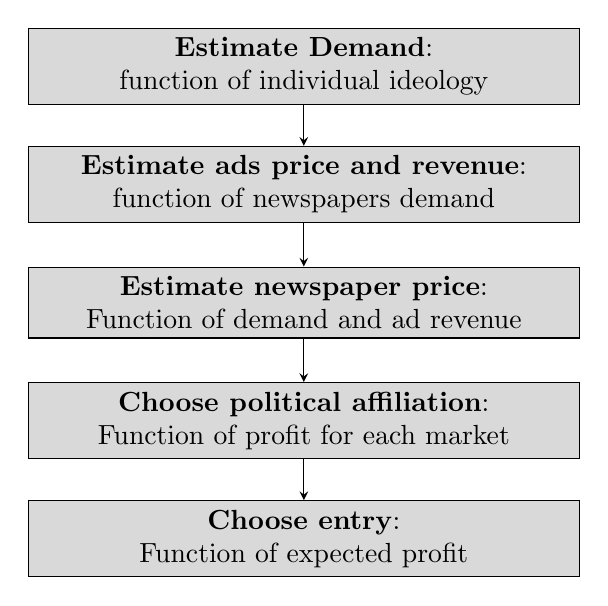
\begin{tikzpicture}[baseline=0, node distance=1.5cm]
    \node (demand) [std, align=center]
      {\textbf{Estimate Demand}: \\ function of individual ideology};
    \node (ads)    [std, below of=demand]
      {\textbf{Estimate ads price and revenue}: \\ function of newspapers
        demand};
    \node (price)  [std, below of=ads]
      {\textbf{Estimate newspaper price}: \\ Function of demand and ad revenue};
    \node (ideo)   [std, below of=price]
      {\textbf{Choose political affiliation}: \\ Function of profit for each
        market};
    \node (entry)  [std, below of=ideo]
      {\textbf{Choose entry}: \\ Function of expected profit};

    \draw [arrow] (demand) -- (ads);
    \draw [arrow] (ads)    -- (price);
    \draw [arrow] (price)  -- (ideo);
    \draw [arrow] (ideo)   -- (entry);
  \end{tikzpicture}
\end{frame}

\begin{frame}[t]{Data}
  \begin{itemize}
    \item For the supply side (Entry and affiliation), data on the number,
      affiliations, and circulation prices of individual newspaper are used.
      \begin{itemize}
        \item Collected from the US Newspaper Panel
      \end{itemize}
    \item For the demand side, data on circulation per town and newspaper
      is used.
      \begin{itemize}
        \item Collect from Audit Bureau of Circulations.
      \end{itemize}
    \item Supplementary datasets on newspaper revenue and costs, alongside
      readership surveys, are used to calibrate the model
    \item \textit{Note: The process of matching data from the different databases
      is complex and a considerable amount of data is lost.}
  \end{itemize}
\end{frame}

\begin{frame}[t]{Data Summary for markets - US Newspaper Panel}
  \begin{figure}
  \begin{center}
    \includegraphics[scale=0.14]{Table1.png}
  \end{center}
  \end{figure}

  \begin{itemize}
    \item Number of papers is highly correlated to population
    \item The share of Republican Newspapers (57\%) is slightly higher than
      the share of Republican votes (51\%)
  \end{itemize}
\end{frame}

\begin{frame}[t]{Data Summary for towns - ABC x Panel}
  \begin{figure}
  \begin{center}
    \includegraphics[scale=0.14]{Table2.png}
  \end{center}
  \end{figure}

  \begin{itemize}
    \item Mostly the same conclusions as before.
    \item Data lost by the matching process causing the share of Republican
      newspaper to fall to (55\%)
  \end{itemize}

\end{frame}

\begin{frame}[t]{Descriptive Evidence}
  \begin{itemize}
    \item Data shows that increasing the fraction Republican among voters
      by 10 percentage points increases the relative circulation of Republican
      papers by 10 percent.
    \item And that adding a second Republican paper to a market with one Republican and one Democratic newspaper reduces the relative circulation of the existing Republican paper by 4\%.
  \end{itemize}
\end{frame}

\begin{frame}[t]{Descriptive Evidence}
  \begin{figure}
  \begin{center}
    \includegraphics[scale=0.15]{Table3.png}
  \end{center}
  \end{figure}
\end{frame}


\begin{frame}[t]{Descriptive Evidence}
  \begin{figure}
  \begin{center}
    \includegraphics[scale=0.15]{Table4.png}
  \end{center}
  \end{figure}
\end{frame}

\begin{frame}[t]{Descriptive Evidence}
  \begin{itemize}
    \item Data shows that a 10 percentage point increase in the fraction of
      Republican among the households increases the likelihood of a Republican
      affiliation by 23\%
    \item But facing a Republican incumbent, instead of a Democratic one,
      reduces the likelihood by 28\%.
  \end{itemize}
\end{frame}

\begin{frame}[t]{Descriptive Evidence: Summary}
  \begin{figure}
  \begin{center}
    \includegraphics[scale=0.17]{Fig1A.png}
  \end{center}
  \end{figure}
\end{frame}

\begin{frame}[t]{Descriptive Evidence: Summary}
  \begin{figure}
  \begin{center}
    \includegraphics[scale=0.17]{Fig1B.png}
  \end{center}
  \end{figure}
\end{frame}

\begin{frame}[t]{Model Setup}
  \begin{itemize}
    \item There are $M$ markets. Each one is indexed by $m \in {1,...,M}$.
    \item Each market has a unit mas of homogeneous advertisers and a mass
      $S_m$ of households. Households are indexed by $i \in {1,...,S_m}$
    \item $J_m$ is the number of newspapers that choose to enter market $m$.
      Newspapers are indexed by $j \in {1,...,J_m}$.
    \item Each entering newspaper choose a political affiliation
      $\tau_{jm} \in \{R,D\}.$
    \item Each household has a political affiliation $\theta_{im} \in \{R, D\}$.
    \item $\rho_m$ represents the share or Republican households within the
      market and is common knowledge.
  \end{itemize}
\end{frame}

\begin{frame}[t]{Model Setup: Consumer problem}
  The household utility function is given by:
  \[ u_{im}(\mathcal{B}) = \sum_{j \in \mathcal{B}}
    (\underline{\beta}\textbf{1}_{\theta_{im} \ne \tau_{jm}}
    + \bar{\beta}\textbf{1}_{\theta_{im} = \tau_{jm}}
    - \alpha p_{jm}) -
    g_s(\mathcal{B})\Gamma_s - g_d(\mathcal{B})\Gamma_d +
    \epsilon_{im}(\mathcal{B}) \]
  where:
  \begin{itemize}
    \item $\mathcal{B}$ is the consumed bundle newspapers,
    \item $p_{jm}$ is the price of newspaper $j$,
    \item $g_s(\mathcal{B})$ is the number of distinct two-newspaper subsets
      of bundle $\mathcal{B}$ such that the two newspaper have the same
      political affiliation,
    \item $g_d(\mathcal{B})$ is the number of distinct two-newspaper subsets
      of bundle $\mathcal{B}$ such that the two newspaper have the different
      political affiliation,
    \item $\epsilon_{im}(\mathcal{B})$ is a type-I extreme value error,
    \item $\epsilon_{im}(\varnothing)$ is the outside good ("No News") utility.
   \end{itemize}
\end{frame}


\begin{frame}[t]{Model Setup: Advertising market}
  The advertiser profit is given by:

  \[ \int_i \textbf{1}_{n_{im} \geq 1}[a_h + (n_{im} - 1)a_l] -
    a_{jm}q_{jm}S_m \]

  Where:
  \begin{itemize}
    \item $n_{im}$ is the number of newspaper read by $i$,
    \item $a_h$ and $a_l$ are the value to advertiser of first and subsequent
      impressions respectively, with $0 \leq a_l \leq a_h$.
  \end{itemize}

\end{frame}

\begin{frame}[t]{Model Setup: Supply}
  Newspapers profit is given by:
  \[ \pi_{jm} = S_m[(p_{jm} + \psi_{jm}a_{jm} - MC)q_{jm} -
    \xi_{jm}(\tau_{jm})] - \kappa_m \]

  Where:
  \begin{itemize}
    \item $\pi_{jm}$ is the profit of newspaper $j$,
    \item $q_{jm}$ is the market share of newspaper $j$, given
      by the previous equation,
    \item $\psi_{jm}$ is the mass of advertisers advertising in newspaper $j$,
    \item $a_{jm}$ is newspaper $j$'s per-copy advertising price,
    \item $MC$ is a marginal cost common to all newspapers and markets,
    \item $\xi_{jm}(\tau_{jm})$ is an affiliation specific cost,
    \item $\kappa_m$ is a market-specific fixed cost.
    \item All above variables are market $m$-specific.
  \end{itemize}
\end{frame}

\begin{frame}[t]{Model Setup: Supply Cont..}
  \begin{itemize}
    \item $\kappa_m/S_m$ is distributed logistic with scale parameter
      $\sigma_\kappa$ and a location parameter
      $\mu_\kappa^0 + \mu_\kappa^1\log(S_m)$.
    \item $\xi_{jm}(\tau_{jm})/\sigma_\xi$ a is distributed mean-zero
      type-I extreme value, where $\sigma_\xi > 0$ is a constant.
  \end{itemize}
\end{frame}

\begin{frame}[t]{Equilibrium}
  An equilibrium is achieved though the 5 step process described before:
  \center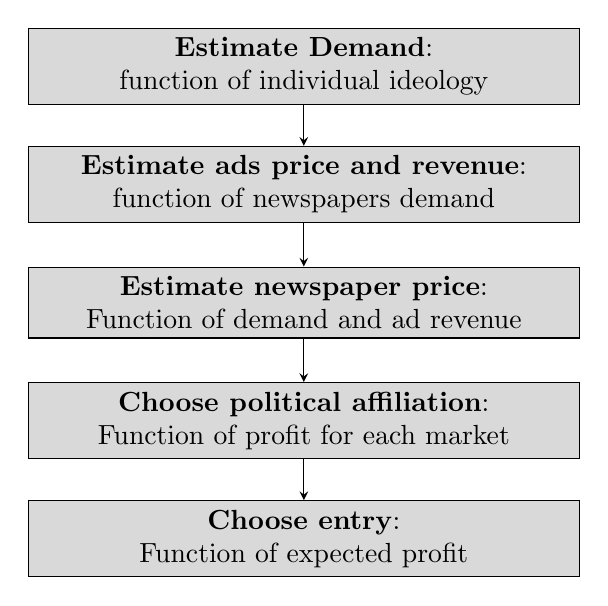
\begin{tikzpicture}[baseline=0, node distance=1.5cm]
    \node (demand) [std, align=center]
      {\textbf{Estimate Demand}: \\ function of individual ideology};
    \node (ads)    [std, below of=demand]
      {\textbf{Estimate ads price and revenue}: \\ function of newspapers
        demand};
    \node (price)  [std, below of=ads]
      {\textbf{Estimate newspaper price}: \\ Function of demand and ad revenue};
    \node (ideo)   [std, below of=price]
      {\textbf{Choose political affiliation}: \\ Function of profit for each
        market};
    \node (entry)  [std, below of=ideo]
      {\textbf{Choose entry}: \\ Function of expected profit};

    \draw [arrow] (demand) -- (ads);
    \draw [arrow] (ads)    -- (price);
    \draw [arrow] (price)  -- (ideo);
    \draw [arrow] (ideo)   -- (entry);
  \end{tikzpicture}
\end{frame}

\begin{frame}[t]{5th and Final Step: Consumer Equilibrium}
  Solving the consumer problem results in the followings market shares:

  \[ q^\theta_{jm} =
    \frac{\sum\limits_{\{\mathcal{B} \in \mathbb{B} : j \in \mathcal{B}\}}
        \exp(u^\theta_m(\mathcal{B}))}
      {\sum\limits_{\mathcal{B}' \in \mathbb{B}} \exp(u^\theta_m(\mathcal{B}'))}
    \]

    Where:
    \begin{itemize}
      \item $q^\theta_{jm}$ is the share of newspaper $j$ among households of
        affiliation $\theta$ in market $m$.
      \item $u^\theta_m(\mathcal{B})$ is the utility for household of
        affiliation $\theta$ of bundle $\mathcal{B}$
      \item $\mathbb{B}$ is the set of all possible newspapers' bundles in
        market $m$.
    \end{itemize}

    Therefore, the final market share is given by:

    \[q_{jm} = \rho_mq^R_{jm} + (1 - \rho_m) q_{jm}\]
\end{frame}

\begin{frame}[t]{4th Step: Advertising Equilibrium}
  \[ a_{jm}(\textbf{p}, \text{\boldmath$\tau$}) = a_h\mathcal{E}_{jm}(\textbf{p},
    \text{\boldmath$\tau$}) + a_l(1 - \mathcal{E}_{jm}(\textbf{p}, \text{\boldmath$\tau$})) \]

  Where:
  \begin{itemize}
    \item $\textbf{p}$ and $\text{\boldmath$\tau$}$ are the price and affiliation vector of newspapers in market $m$,
    \item $\mathcal{E}_{jm}$ is the share of newspaper j's that are exclusive,
    \item Note: this is simply a pondered mean of exclusive and non-exclusive
      advertasing prices,
    \item It is not clear to me how $ \mathcal{E}_{jm}$ is estimated.
  \end{itemize}
\end{frame}

\begin{frame}[t]{3th Step: Newspaper price}
  \[ p^*_j \in \arg\max_{p_j} (p_j + a_{jm}(\textbf{p}^*, \text{\boldmath$\tau$})
    - MC)q_{jm}(\textbf{p}^*, \text{\boldmath$\tau$}) \]

  \begin{itemize}
    \item Given demand and ad price, choose newspaper price to maximize profit,
    \item A proof of the uniqueness for optimal price in not provide. Matlab doesn't
      care and neither do the authors.
  \end{itemize}
\end{frame}

\begin{frame}[t]{2th Step: Newspaper price}
  \begin{itemize}
    \item Firms now sequentially choose affiliations given the number of newspapers
      and their affiliation-specific shocks.
    \item That is: given expected profits, firms choose affiliations.
    \item Formally:
  \end{itemize}

  \[ \tau^*_j = \arg\max_{\tau} E_{\tau^*_{j^+}} [\nu_{jm}([
      \text{\boldmath$\tau$}^*_{j^-}, \tau,\text{\boldmath$\tau$}^*_{j^+}])
      - \xi_{jm}(\tau^*_j))] \]

    Where:
    \begin{itemize}
      \item $\nu_{jm}$ is the equilibrium value for $(p_{jm} + a_{jm} - MC)q_{jm}$
    \end{itemize}
\end{frame}

\begin{frame}[t]{1th Step: Entry}
  Finally firms decide either to enter or not. The per-household
  expected variable profit is:

  \[ V_m(J) = \frac{1}{J} \sum^J_{j = 1} \sum_{\text{\boldmath$\tau$} \in
      \mathcal{T}_J} ( \nu_{jm}(\text{\boldmath$\tau$}) - \bar\xi_{jm}
      (\text{\boldmath$\tau$})) P_m(\text{\boldmath$\tau$}) \]

    \begin{itemize}
      \item where $\mathcal{T}_J$ is the set of \boldmath$\tau$ vectors with
        $|\text{\boldmath$\tau$}| = J$.
    \end{itemize}
    Therefore, if $V_m$ is strictly decreasing in $J$, the decision rule:

    \[ V_m(J^*) \ge \frac{\kappa_m}{S_m} > V_m(J^* + 1) \]

    \begin{itemize}
      \item In other words, firms entries if profit is greater than zero
      \item We can't prove that $V_m$ is strictly decreasing, that is not
        a problem though because it is \textbf{intuitive}
    \end{itemize}
\end{frame}

\begin{frame}[t]{Demand Estimation}
  Remember, we have:
  \begin{itemize}
    \item Newspaper circulation per town ($Q_{jt}$)
    \item Town population ($S_t$)
    \item Republican vote share per town ($Z_t$)
  \end{itemize}

  We need:
  \begin{itemize}
    \item Newspaper market share ($q_{jt}$)
    \item Republican affiliation share - household ($\rho_t$)
    \item Republican affiliation share - newspaper ($\tau_{jt}$)
  \end{itemize}

  In order to find the parameters that makes:

  \[ q^\theta_{jm} =
    \frac{\sum\limits_{\{\mathcal{B} \in \mathbb{B} : j \in \mathcal{B}\}}
        \exp(u^\theta_m(\mathcal{B}))}
      {\sum\limits_{\mathcal{B}' \in \mathbb{B}} \exp(u^\theta_m(\mathcal{B}'))}
    \]
\end{frame}

\begin{frame}[t]{Demand Estimation}
  We assume that:

  \[ Q_{jt} = q_{jt}S_t\zeta_{jt} \]

  Where:
  \begin{itemize}
    \item $log \zeta_{jt} \sim N(0, \sigma^2_\zeta)$ is a measurement error.
  \end{itemize}

  And estimate $\rho_t$ and $\tau_{jt}$, by:

  \[ \rho_t = \logit^{-1}(\logit(Z_t) + \nu_t) \]
  \[ Pr( \tau_{jt} = R ) = \logit^{-1}( \mu^0_\rho + \mu^1_\rho \logit(\rho_t)) \]

  Where:
  \begin{itemize}
    \item $\nu_t$ is a normally distributed error term with mean 
      $\mu^{\text{town}}_{ \nu}$ and standard deviation 
      $\sigma^{\text{town}}_\nu$.
    \item $\mu^0_\rho$ and $\mu^1_\rho$ are parameters to me estimated
    \item the double logit ensures that the numbers are between $(0, 1)$
    %\item $\nu_t$ is assumed to be correlated between pairs of neighbors but 
      %independent across pairs,  with the within-pair correlation restricted to:
  \end{itemize}

  %\[ \frac{\cov(\nu_t, \nu_{t'})}{\var(\nu_t)} = \frac{\cov(\logit(Z_t),
      %\logit(Z_{t'}))}{\var(\logit(Z_t))} \]
\end{frame}

\begin{frame}[t]{Demand Estimation - Notes}
  \begin{itemize}
    \item Note that we don't use the affiliation strategy described in the equilibrium section.
    That is because that strategy is only valid in the newspaper headquarter market
    and not in the hinterland tows whose data is used to estimate demand.
  \item Headquarter markets are ignored in demand estimation because reasons other
    than political affiliation is assumed to dominate the demand function.
  \end{itemize}

\end{frame}

\begin{frame}[t]{Demand Estimation}
  Then, the conditional likelihood of the data for town $t$ is:

  \small\[
    L_t(\rho_t) = \frac{1}{\tilde\sigma_t} \phi\left(
    \frac{1}{\tilde\sigma_t|\mathcal{J}^R_t|}
    \sum_{j \in \mathcal{J}^R_t} \log( \frac{\hat{Q}_{jt}}{q_{jt}}) - 
    \frac{1}{\tilde\sigma_t|\mathcal{J}^D_t|}
    \sum_{j \in \mathcal{J}^D_t} \log( \frac{\hat{Q}_{jt}}{q_{jt}})
    \right)Pr(\text{\boldmath$\tau$} | \rho_t, J_t)
  \]

  Where:
  \begin{itemize}
    \item $\tilde\sigma_t = \sigma_\zeta\sqrt{1/|\mathcal{J}^R_t| 
        + 1/|\mathcal{J}^D_t|}$ 
  \end{itemize}

  The unconditional log likelihood of the observed data is:

  \[
    \log L = \sum_{t, t'} \log\int_{\rho_t, \rho_{t'}} L_t(\rho_t)L_{t'}(\rho_{t'}) 
    dF^{\text{town}}(\rho_t,\rho_{t'} | Z_t, Z_{t'})
  \]

  We choose parameters $\{\bar\beta,\Gamma_s, \sigma_\zeta, \mu^{\text{town}}_\nu, 
    \sigma^{\text{town}}_\nu, \mu^0_\rho, \mu^1_\rho\}$ to maximize above log
  likelihood.
\end{frame}

\begin{frame}[t]{Demand Estimation}
  \begin{itemize}
    \item We are still left to estimate the demand parameters $\alpha, 
      \underline{\beta}, \Gamma_d$
    \item To estimate this parameters we first estimated $MC$ and $a_h$ using
      Revenue and Cost data.
    \item Then choose the price coefficient $\alpha$ and the utility shifter
      $\underline\beta$ so that the predicted average price and circulation per
      household match the data
    \item Finally we choose the subtitution parameter $\Gamma_d$ so that the
      predicted overlap in readership matches the data.
  \end{itemize}
\end{frame}

\begin{frame}[t]{Supply Estimation}
  We now observe:
  \begin{itemize}
    \item Market population ($S_m$),
    \item Republican vote share per market ($Z_m$),
    \item Number of newspaper entrants ($J_m$),
    \item Affiliation choices $\tau_m$.
  \end{itemize}

  And we need:
  \begin{itemize}
    \item Republican affiliation share ($\rho_m$)
  \end{itemize}

  To find the parameters that best fit the number of observed entrants $J_m$ to
  the one estimated by the model:

    \[ J^* \text{ such that } V_m(J^*) \ge \frac{\kappa_m}{S_m} > V_m(J^* + 1) \]

\end{frame}
  
\begin{frame}
  The conditional likelihood of the data for market $m$ is:

  \small\[
    L_m(\rho_m) = \begin{cases}
      1 - G_m(V(J_m + 1, \rho)), &\text{ if }J_m = 0 \\
      [G_m(V(J_m,\rho_m)) - G_m(V(J_m + 1,\rho_m))]
      Pr(\text{\boldmath$\tau$}_m, \rho_m) &\text{ if } J_m > 0
    \end{cases}
  \]

  Where:
  \begin{itemize}
    \item $G_m$ is the CDF of $\kappa_m/S_m$
  \end{itemize}

  Therefore the unconditional log likelihood is:

  \[
    \log L = \sum_{(m, m')} \log\int_{\rho_m, \rho_{m'}} L_m(\rho_m)L_{m'}(\rho_{m'})
    dF^{\text{mkt}}(\rho_m, \rho_{m'} | Z_m, Z_{m'})
  \]

  And the parameters $\{a_l, \sigma_\xi, \mu^{\text{mkt}}_\nu, \sigma^{\text{mkt}}_\nu,
  \mu^0_\kappa, \mu^1_\kappa, \sigma_\kappa\}$ are chosen to maximize above likelihood.
\end{frame}

\begin{frame}[t]{Results - Demand Estimation}
  \begin{figure}
  \begin{center}
    \includegraphics[scale=0.19]{Table5.png}
  \end{center}
  \end{figure}
\end{frame}

\begin{frame}[t]{Results - Demand Estimation}
  Highlights:
  \begin{itemize}
    \item Price coefficient ($\alpha$) is positive and significant,
    \item Utility from same affiliation paper ($\bar\beta$) is positive and significant,
    \item Utility from different affiliation paper ($\underline\beta$) is negative
      and significant,
    \item $\Gamma_d$ and $\Gamma_s$ are both positive and significant (Diminishing
      return holds).
  \end{itemize}

  Therefore the model holds as expected!
\end{frame}

\begin{frame}[t]{Results - Supply Estimation}
  \begin{figure}
  \begin{center}
    \includegraphics[scale=0.15]{Table6.png}
  \end{center}
  \end{figure}
\end{frame}

\begin{frame}[t]{Results - Supply Estimation}
  Highlights:
  \begin{itemize}
    \item $a_h$ is "significantly" (?) higher than $a_l$
  \end{itemize}

  Also as expected.
\end{frame}

\begin{frame}[t]{Results - Relevance}
  \begin{figure}
  \begin{center}
    \includegraphics[scale=0.15]{Table7.png}
  \end{center}
  \end{figure}

  \begin{itemize}
    \item To interpret the relevance of our parameters alternative scenarios are
      simulated,
    \item Table 7 shows that our parameters of interest have a dramatic effect
      on the simulations,
    \item The effect of idiosyncratic cost shocks (the residual term) is 
      less relevant.
  \end{itemize}
\end{frame}

\begin{frame}[t]{Results - What would a social planner do?}
  \begin{figure}
  \begin{center}
    \includegraphics[scale=0.15]{Table8.png}
  \end{center}
  \end{figure}
\end{frame}

\begin{frame}[t]{Results - What would a social planner do?}
  \begin{itemize}
    \item To maximize Total Surplus the Social planner lower newspaper price to
      almost zero, expand the reach and diversity of the market.
    \item That is, in the Baseline model we have insufficient entry of newspapers.
    \item What is the best policy to minimize this inefficiency?
  \end{itemize}
\end{frame}

\begin{frame}[t]{Results - Policy}
  \begin{figure}
  \begin{center}
    \includegraphics[scale=0.15]{Table9.png}
  \end{center}
  \end{figure}
\end{frame}

\begin{frame}[t]{Results - Policy}
  \begin{itemize}
    \item Allowing price collusion reduces economic welfare and has little effect on
      diversity.
    \item Advertising collusion, on the other hand, causes large increases in both
      economic welfare and diversity.
    \item Joint operation, which combines the effect of price collusion and 
      advertising collusion, has a overall positive effect on diversity but a
      neutral effect on welfare.
    \item Joint ownership significantly reduces welfare, diversity, and the number
      of newspapers.
    \item A marginal cost subsidy, that is a transfer of K dollars per newspaper sold,
      reveals the greatest increase in total surplus.
  \end{itemize}
\end{frame}

\begin{frame}[t]{Conclusions}
  \begin{itemize}
    \item Competitive incentives are a crucial driver of ideological diversity,
    \item There is no conflict between the goal of maximizing economic welfare
      and the goal of preserving ideological diversity,
    \item It's important to distinguish between advertising collusion, which
      has a positive effect on welfare and diversity, price collusion, which has 
      mixed effects, and joint operation, which is inferior to advertising collusion.
  \end{itemize}
\end{frame}

\end{document}
